\chapter{Data}
\label{ch:data}

\section{Study area}

Aberfoyle Forest lies within Queen Elizabeth Forest Park, Trossachs National Park, Scotland, near OS grid reference NN~520~010. The forest extent is roughly 20\,km by 15\,km, with plots clustered by management compartment. Elevation ranges from about 25\,m at the valley floor to over 500\,m on the ridges, with steep glens, exposed ridges, and lochs. Exact plot or grid-cell size is not yet confirmed from Forest Research metadata; records are treated as spatial polygons or centroids in OSGB36.

\section{LiDAR-derived plot data}
\label{sec:data-lidar}

Plot-level attributes come from airborne LiDAR surveys at six timestamps: 2002, 2006, 2008, 2012, 2021, and 2023. The acquisition platform is not confirmed in the available metadata, so this dissertation says airborne LiDAR-derived plot attributes rather than assuming a specific platform such as drone or fixed-wing.

Two local data sources exist and should not be confused. A legacy CSV export (\texttt{LiDAR\_Years\_All\_attributes.csv}, dated 29 June) has 1,152,801 rows and 23 columns. The current working source is a GeoPackage (\texttt{LiDAR\_Years\_All\_7jul.gpkg}) with two layers: \texttt{LiDAR\_Years} (795,645 rows, 40 fields plus geometry) and \texttt{LiDAR\_Years\_SS}, a Sitka-spruce-filtered subset (376,080 rows). All cohorts below come from the GeoPackage, not the legacy CSV.

The main response variable is \texttt{Top\_Height95}, defined as \texttt{elev\_percentile\_95th} times 1.1. A related field, \texttt{Top\_Height99}, comes from the 99th elevation percentile without a multiplier, so \texttt{Top\_Height99} is lower than \texttt{Top\_Height95} in many rows. This dissertation uses \texttt{Top\_Height95} as the response and \texttt{Top\_Height99} only for audit checks.

\section{Cleaning decisions}

Cleaning is applied at plot level after fixing a required set of cohort years. A plot is kept only if it passes every rule in every required year, so the result stays balanced across timestamps. The rules: keep the required years; keep plots present in every required year; filter to Sitka spruce with \texttt{spis == "SS"}, since \texttt{spis} is the Forest Research species code and disagrees with the separate \texttt{Species} field; keep valid planting years; keep plausible age (\texttt{Age = LiDAR\_year - plyr}); and keep plausible \texttt{Top\_Height95} values. Volume is not part of general cleaning; negative \texttt{Vol\_RM95} values stay in the master export and are filtered only in volume-specific analyses.

\section{Cleaned cohorts}

Two balanced Sitka spruce cohorts result. The four-survey cohort covers 2008, 2012, 2021, and 2023: 71,766 plots, 287,064 rows. The six-survey cohort covers all six years: 13,897 plots, 83,382 rows. The four-survey cohort is the main dataset, since it is roughly five times larger. The six-survey cohort is used for full-span sensitivity checks and the temporal question, since only it spans 21 years.

\begin{table}[h]
\centering
\begin{tabular}{lrrl}
\toprule
Cohort & Plots & Rows & Survey years \\
\midrule
Four-survey (main) & 71,766 & 287,064 & 2008, 2012, 2021, 2023 \\
Six-survey (sensitivity) & 13,897 & 83,382 & 2002, 2006, 2008, 2012, 2021, 2023 \\
\bottomrule
\end{tabular}
\caption{Cleaned Sitka spruce cohorts used for modelling.}
\label{tab:cohorts}
\end{table}

Each cleaning rule removes plots unevenly across the forest -- the Sitka spruce filter and the age filter tend to remove whole compartments, not a random scatter. Figure~\ref{fig:cleaning-stages} shows this cumulative effect on an earlier four-year cohort extract.

\begin{figure}[h]
\centering
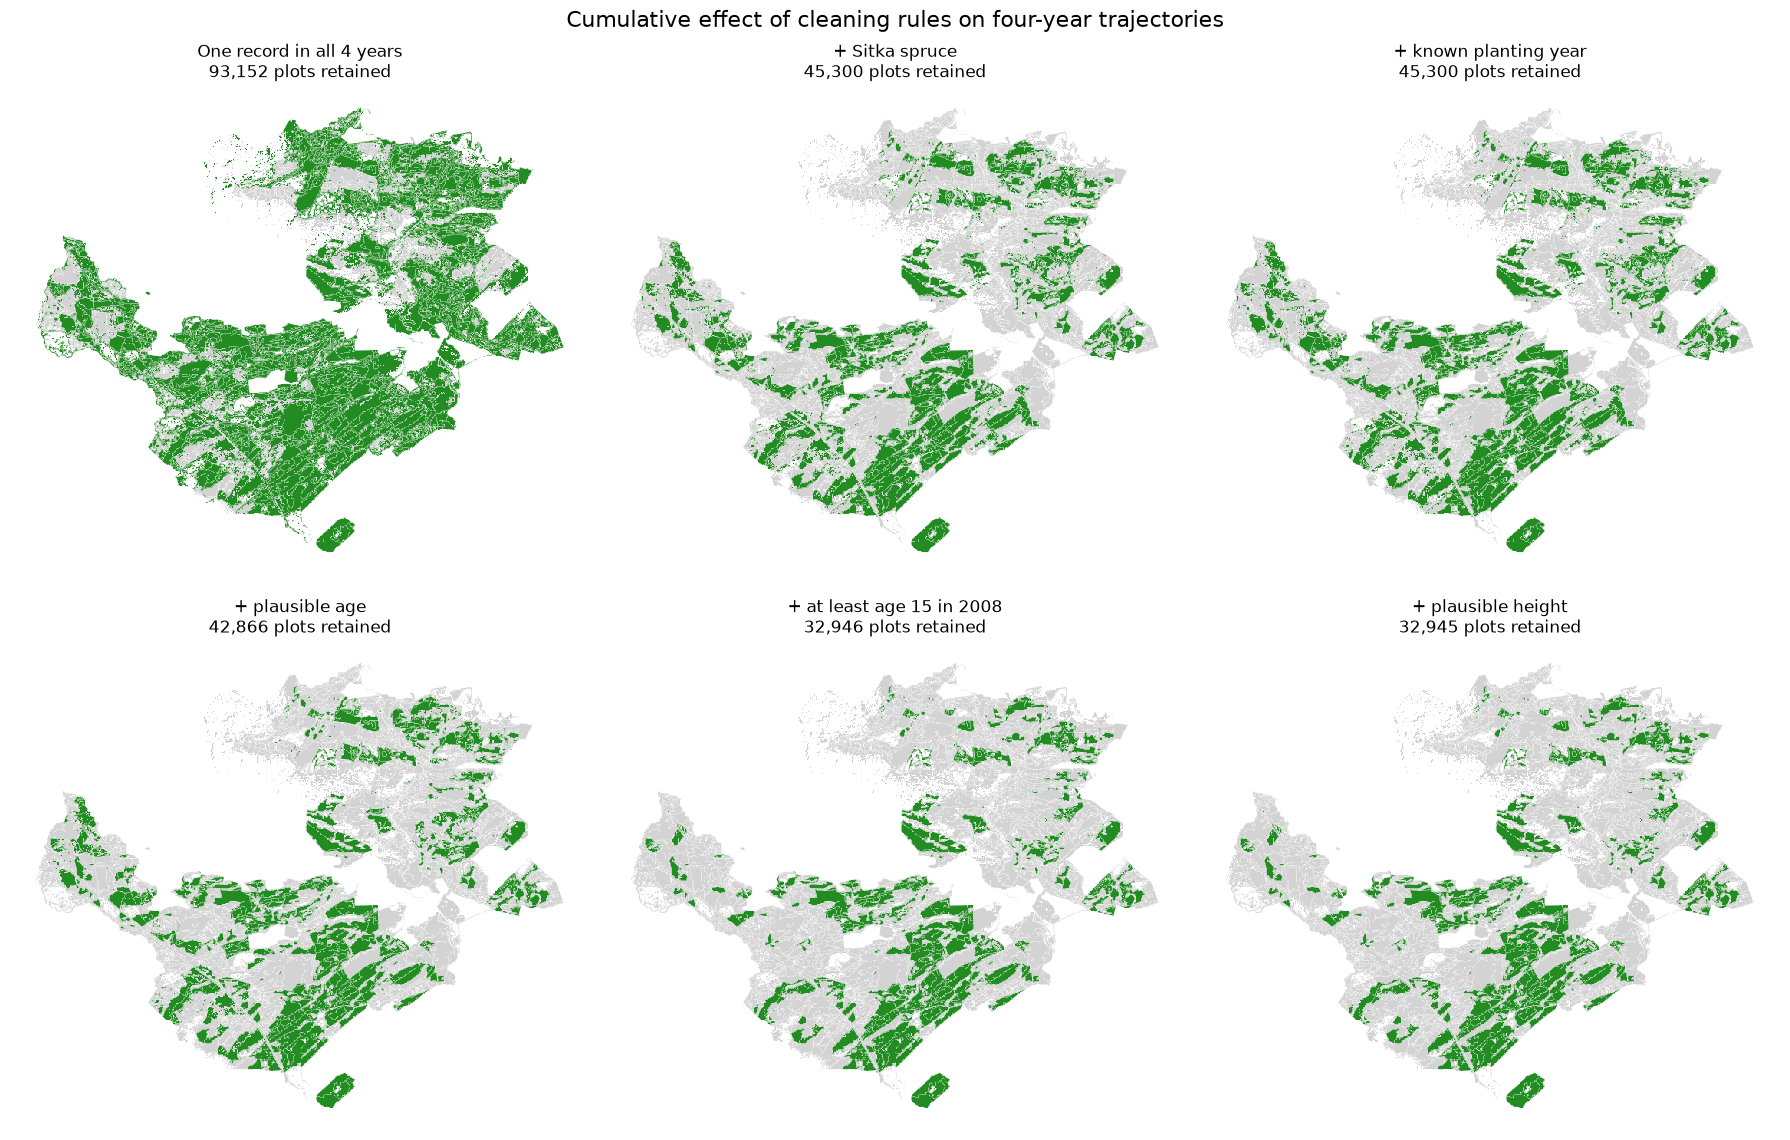
\includegraphics[width=\textwidth]{figures/legacy_examples/cleaning_stages_map_example.png}
\caption{Example figure from an earlier Aberfoyle dataset/workflow. Included to illustrate the planned analysis; not a final result. Cumulative spatial effect of the cleaning rules on an earlier four-year cohort extract (retained plots in green, removed in grey). Plot counts and geometry do not match the current cohorts in Table~\ref{tab:cohorts}.}
\label{fig:cleaning-stages}
\end{figure}

\section{Response variable and Chapman-Richards residuals}

The response is \texttt{Top\_Height95}. CR parameters ($y_{\max}$, $k$, $p$) are fitted once, by least squares, using \texttt{Age} as the time input across all plot-timestamp pairs. The residual for plot $i$ at time $t$ is
\[
\varepsilon_{i,t} = y_{i,t}^{\text{obs}} - y_{\text{CR}}(t_i \mid y_{\max}, k, p),
\]
where a positive value means the plot is taller than the age-matched CR baseline, and a negative value means shorter. This fit has not yet run on the current cohorts; Chapter~\ref{ch:results} reports placeholders until it does.

\section{Terrain, wind, climate, and soil data}

Terrain variables -- elevation, slope, northness, eastness, TWI, and TOPEX -- will come from the OS Terrain 50 DTM \citep{osdatahub2026OSTerrain50} (50\,m post spacing) at each plot centroid, using \texttt{rasterio} and \texttt{geopandas}. WASP wind data will be added if available with a documented resolution; otherwise the Global Wind Atlas \citep{globalwindatlas2026GlobalWindAtlas} (250\,m grid) serves as a public fallback, using the lowest above-ground height relevant to canopy exposure. None of this extraction has run yet.

HadUK-Grid \citep{hollis2019HadUKGridGriddedClimate} gives 1\,km gridded daily UK climate data, used for interval-level indices such as summer soil moisture deficit and growing degree days, one value per survey interval. At 1\,km it is coarse next to plot scale, so it is a temporal signal, not a spatial predictor, unless extraction shows real within-forest variation. Soil data is treated the same way: included only if it shows enough unique values inside Aberfoyle to distinguish nearby plots. Neither has been extracted yet.

\section{Leakage risks and excluded variables}
\label{sec:data-leakage}

Some GeoPackage fields are derived from height, age, or both, and would leak the target. These are excluded from all predictor sets: \texttt{Vol95}, \texttt{Vol99}, \texttt{Vol\_RM95} (from height, area, canopy cover), \texttt{GYCspec95} and \texttt{GYCspec99} (from height and age, with some infinite or extreme values), the raw height percentiles, and \texttt{Top\_Height99}.

\texttt{whcl} is a Forest Research windthrow hazard class, not a raw wind measurement, and looks management-linked: plots with \texttt{whcl > 4} are thinned in only 2.63\% of records (312 plots), and class 6 is almost entirely unthinned. It is kept for audit only.

Management fields (\texttt{Thin}, \texttt{last\_thinn}, \texttt{time\_since\_thinning}) are useful context but not a substitute for terrain and wind attribution: \texttt{Thin} only records whether a last-thinning year exists, not whether it affected the observed interval. Thinning is the main unobserved confounder, discussed further in Chapter~\ref{ch:discussion}.

\section{Multicollinearity}

A correlation matrix and variance inflation factor (VIF) check are planned before modelling, since elevation, TOPEX, and any wind layer likely overlap. Figure~\ref{fig:correlation-example} shows the intended format. XGBoost should handle correlated predictors implicitly; the linear baseline will drop the more redundant variable in pairs with VIF above 10.

\begin{figure}[h]
\centering
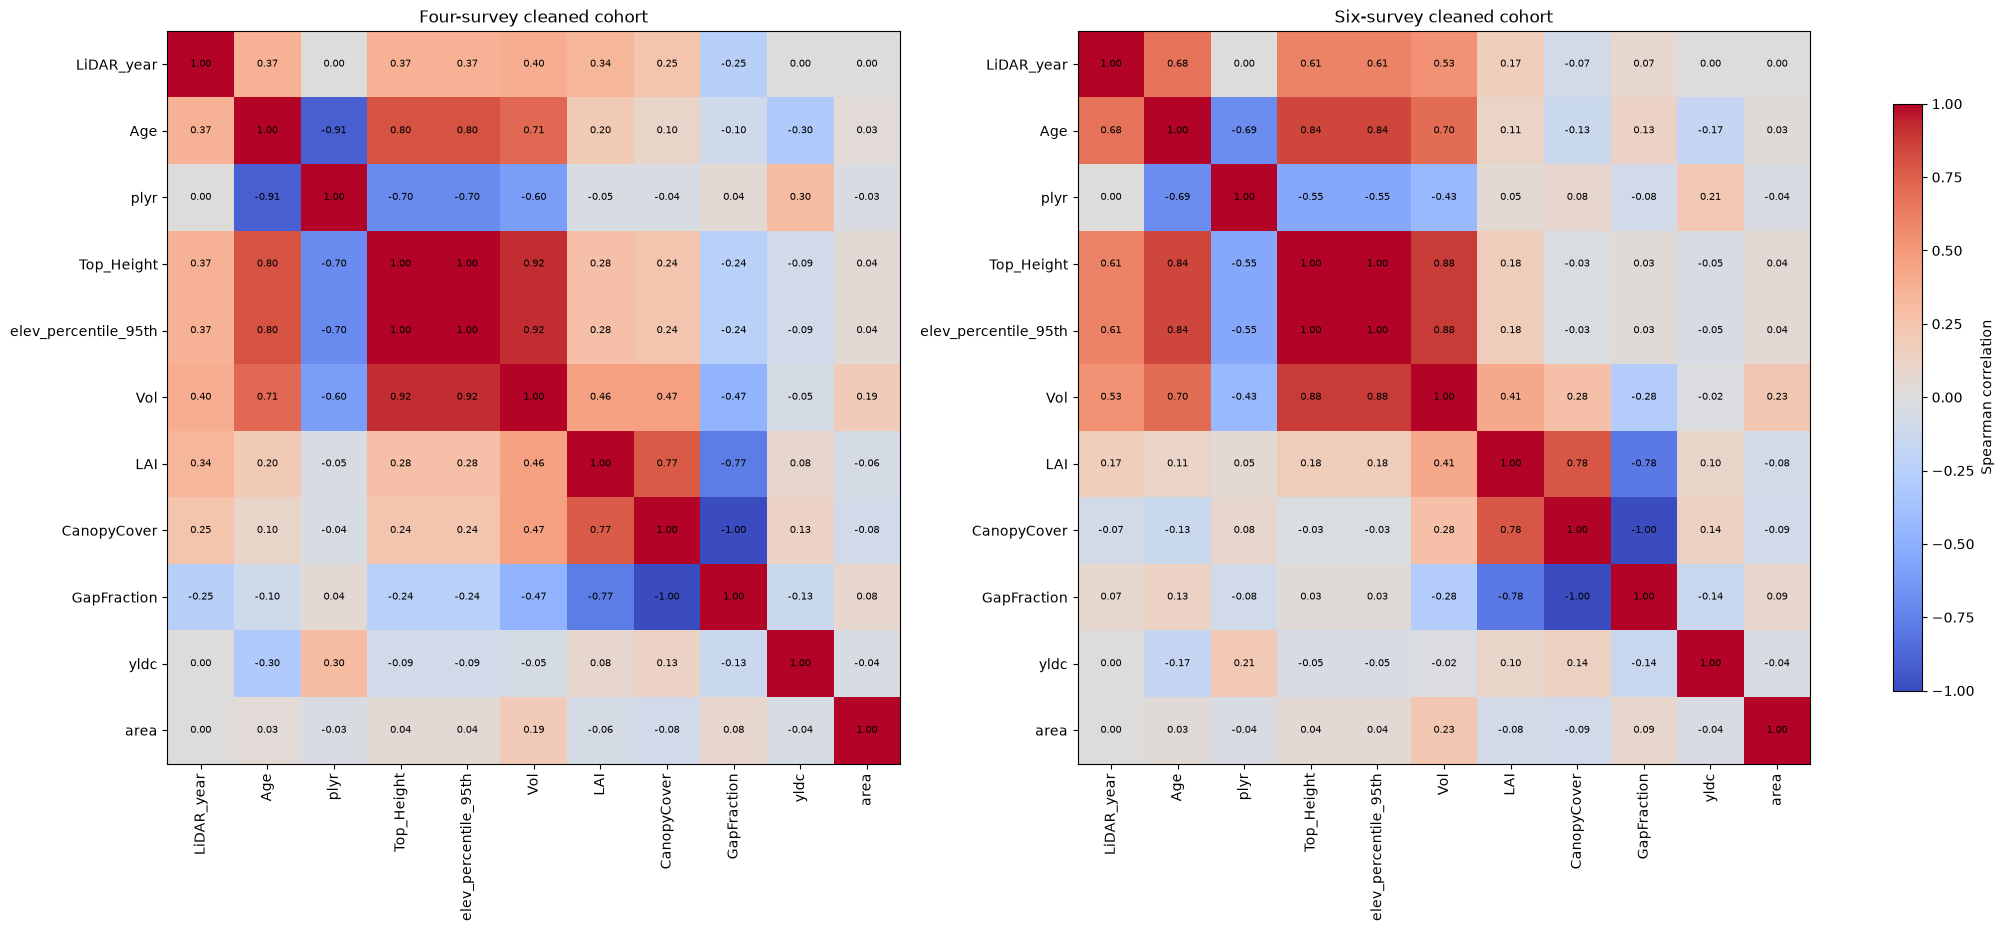
\includegraphics[width=\textwidth]{figures/legacy_examples/correlation_matrix_example.png}
\caption{Example figure from an earlier Aberfoyle dataset/workflow. Included to illustrate the planned analysis; not a final result. Spearman correlation matrix for the four-survey and six-survey cohorts from an earlier cleaning pass, before terrain and wind features were joined.}
\label{fig:correlation-example}
\end{figure}
